\documentclass[11pt]{article}

\usepackage[letterpaper,margin=1in]{geometry}
\usepackage[T1]{fontenc}
\usepackage[utf8]{inputenc}
\usepackage{lmodern}
\usepackage{microtype}
\usepackage{xcolor}
\usepackage{graphicx}
\usepackage{booktabs}
\usepackage{tabularx}
\usepackage{longtable}
\usepackage{array}
\usepackage{enumitem}
\usepackage{fancyhdr}
\usepackage{titlesec}
\usepackage{tikz}
\usetikzlibrary{arrows.meta,positioning,shapes.geometric}
\usepackage[hidelinks]{hyperref}

\definecolor{SabayTerracotta}{HTML}{C96543}
\definecolor{SabayBrown}{HTML}{6F4E37}
\definecolor{SabayCream}{HTML}{FAF4ED}
\definecolor{SabayGray}{HTML}{555555}

\hypersetup{
  pdftitle={SF2026 Capstone: Connecting Communities with Sabay},
  pdfauthor={Christopher Kuttruff, Ethan Dibble, Olga Ishimwe, Sefu Alvarez, Vincent Le},
  colorlinks=true,
  linkcolor=SabayBrown,
  urlcolor=SabayTerracotta
}

\pagestyle{fancy}
\fancyhf{}
\lhead{Sabay Capstone Project Document}
\rhead{SF2026}
\cfoot{\thepage}
\setlength{\headheight}{14pt}
\setlength{\parindent}{0pt}
\setlength{\parskip}{0.65em}
\setlist{nosep,leftmargin=1.5em}
\titleformat{\section}{\Large\bfseries\color{SabayBrown}}{\thesection}{0.65em}{}
\titleformat{\subsection}{\large\bfseries\color{SabayTerracotta}}{\thesubsection}{0.65em}{}

\newcommand{\TBD}[1]{\textcolor{SabayTerracotta}{\textbf{Team input needed:} #1}}
\newcommand{\status}[1]{\textsc{#1}}

\begin{document}

\hypersetup{pageanchor=false}
\begin{titlepage}
  \pagecolor{SabayCream}
  \color{SabayBrown}
  \centering
  \vspace*{1.1in}
  {\Huge\bfseries SF2026 Capstone:\par}
  \vspace{0.18in}
  {\Huge\bfseries Connecting Communities with Sabay\par}
  \vspace{0.35in}
  {\Large A community resource for trusted support at home\par}
  \vfill
  {\large Portland State University\par}
  {\large Computer Science Capstone\par}
  \vspace{0.4in}
  \begin{tabular}{c}
    Christopher Kuttruff \\
    Ethan Dibble \\
    Olga Ishimwe \\
    Sefu Alvarez \\
    Vincent Le
  \end{tabular}
  \vspace{0.45in}

  {\large August 20, 2026\par}
  \vspace{0.7in}
  {\small Implementation plan for the following academic term\par}
  \pagecolor{white}
\end{titlepage}

\hypersetup{pageanchor=true}
\pagenumbering{arabic}

\section{Project Metadata}

\begin{tabularx}{\textwidth}{>{\bfseries}p{0.28\textwidth}X}
\toprule
Title & SF2026 Capstone: Connecting Communities with Sabay \\
Date & August 20, 2026 \\
University and program & Portland State University Computer Science Capstone \\
Capstone cycle & SF2026 \\
Team members & Christopher Kuttruff; Ethan Dibble; Olga Ishimwe; Sefu Alvarez; Vincent Le \\
Sponsor & Erin Meneley (inferred from the project proposal; confirmation needed) \\
Supervisor & Bruce Irvin\\
Source code & \url{https://github.com/sabay-org/sabay} \\
License & MIT License \\
\bottomrule
\end{tabularx}

\subsection{Responsibilities}

\begin{tabularx}{\textwidth}{p{0.25\textwidth}X}
\toprule
\textbf{Team member} & \textbf{Primary responsibilities} \\
\midrule
Christopher Kuttruff & Team lead, coordination with sponsor, project planning, DevOps, database schema design, back-end functionality \\
Ethan Dibble & TBD \\
Olga Ishimwe & TBD \\
Sefu Alvarez & TBD \\
Vincent Le   & TBD \\
\bottomrule
\end{tabularx}

\section{Why: Purpose and Motivation}

\textbf{Planning context.} This document is the team's high-level plan for the following academic term. It translates sponsor Erin Meneley's objectives into proposed scope, architecture, process, risks, and milestones. The existing repository is the technical baseline; the community-platform capabilities described below are upcoming work unless explicitly marked complete.

\subsection{Sponsor vision}

Sabay---a Filipino word meaning ``together''---will serve as a community-oriented resource connecting aging, ailing, or recovering people and their families with trusted local helpers and caregivers. The sponsor's primary goal is to make reliable in-person support easier to find and coordinate. In doing so, Sabay can also help caregivers contribute their skills through flexible, meaningful service opportunities.

The proposal is grounded in the sponsor's experience helping community members with groceries, transportation, appointments, and household errands. These everyday services can help a person remain safely at home during the period between full independence and assisted living or nursing care. Similar needs arise during recovery from surgery, treatment for serious illness, or episodes of chronic illness.

\subsection{Human problem}

Demand for non-medical, in-person support is high, but families lack a simple, affordable, trusted way to find appropriate caregivers, coordinate work, and remain informed. Informal coordination places another substantial responsibility on relatives who may already be balancing work, family, and care duties. Caregivers, meanwhile, need a way to find suitable work that fits their skills, location, and availability.

Sabay addresses this gap through discovery, trust signals, scheduling, communication, and practical service coordination in one accessible resource.

\subsection{Product principles}

\begin{itemize}
  \item \textbf{Trust and safety:} caregiver review, credential information, clear identity and account controls, and auditable interactions.
  \item \textbf{Ease of use:} a responsive, mobile-friendly interface usable by older adults and people with limited technical experience.
  \item \textbf{Connection:} direct, timely coordination among care seekers, family members, and helpers.
  \item \textbf{Community service before commerce:} product decisions should prioritize access, dignity, trust, and useful support rather than maximizing transactions or revenue.
  \item \textbf{Practical independence:} support for everyday tasks that helps people remain at home longer.
  \item \textbf{Respectful scope:} clear separation between non-medical services and regulated clinical care.
\end{itemize}

\section{What: Functionality and Deliverables}

\subsection{Users}

\begin{description}[style=nextline]
  \item[Care seeker] A person seeking support for themself, such as an older adult, a person with chronic illness, or someone recovering at home.
  \item[Family coordinator] A relative or trusted person who searches, books, communicates, and follows care activity for another person.
  \item[Caregiver/helper] A community member offering non-medical support and managing a profile, qualifications, service opportunities, availability, and compensation where applicable.
  \item[Platform administrator] A Sabay operator who reviews caregiver profiles and verification evidence, moderates activity, and supports users.
\end{description}

\subsection{MVP feature scope}

The mid-project slides describe the MVP as a responsive platform serving both those seeking support and those providing it, with the following capabilities:

\begin{enumerate}
  \item accounts for care seekers and caregivers;
  \item caregiver/service listings with basic search;
  \item booking and scheduling, including the proposal's recurring-task need;
  \item in-app messaging between users;
  \item manual caregiver verification by an administrator;
  \item payment processing; and
  \item notifications for new messages or booking activity.
\end{enumerate}

The mockups add useful product direction: ZIP-code and service-category search; caregiver profiles with ratings, certifications, and background-check indicators; requests for support and caregiver responses; profile comparison and reviews; and service categories including household tasks, errands and shopping, meal preparation, transportation, companionship, post-surgery care, pet care, and technology assistance. They also depict membership plans and video interviews. These mockup elements require sponsor prioritization before they are treated as committed MVP scope, particularly where a commercial model could affect access to the community resource.

\subsection{Current implementation status}

As of August 20, 2026, the repository is an early Django scaffold, not yet the community platform described above. It contains a shared base template, a landing-page view, Simple.css styling, SQLite development configuration, Django's built-in administration route, basic page/static-file tests, Ruff formatting and lint configuration, and GitHub Actions checks.

\subsection{Constraints and assumptions}

\begin{itemize}
  \item The sponsor requires the software to use the MIT open-source license; the repository includes that license.
  \item The team has selected Python and Django. The current scaffold uses Django 6.0.7 and SQLite for local development.
  \item The primary deliverable is a responsive, mobile-friendly web application.
  \item The experience must remain understandable to older or less technical users. Accessibility, readable typography, plain language, large targets, keyboard operation, and mobile layouts should be acceptance criteria rather than late-stage polish.
  \item Care is described as home services and non-medical support.
  \item Safety-sensitive functions such as background checks, credential verification, payments, and emergency handling will depend on third-party services and sponsor policy decisions.
\end{itemize}

\subsection{Planned delivery for the following term}

During the following term, the team plans to implement and validate the sponsor-approved key objectives as a coherent MVP. The expected technical handoff should include the GitHub repository, setup and deployment documentation, automated tests, the final project document, and a working demonstration deployment. We have already established a domain (sabay.org) and a cloud server through Vultr for production deployments. We will automate deployment via Github Actions CICD.

\section{What: Essential User Stories}

The following stories translate the proposal, slides, and mockups into concise user-centered behavior.

\begin{enumerate}
  \item \textbf{Create an account.} As a care seeker or caregiver, I can create and securely access an account so that I can use personalized platform features.
  \item \textbf{Describe care needs.} As a care seeker or family coordinator, I can post the services, location, schedule, and relevant preferences I need so that suitable caregivers can respond.
  \item \textbf{Find caregivers.} As a care seeker or family coordinator, I can search by service and ZIP code so that I can discover nearby helpers.
  \item \textbf{Evaluate a caregiver.} As a care seeker or family coordinator, I can review a caregiver's profile, experience, services, ratings, certifications, and verification status so that I can make an informed choice.
  \item \textbf{Offer services.} As a caregiver, I can maintain my profile, offered services, qualifications, service area, and availability so that care seekers can determine whether I am a match.
  \item \textbf{Respond to a request.} As a caregiver, I can find and respond to suitable requests for support so that I can contribute my skills through flexible, meaningful service.
  \item \textbf{Book support.} As a care seeker or family coordinator, I can request and schedule one-time or recurring support so that both parties agree on when care will occur.
  \item \textbf{Communicate privately.} As a care seeker, family coordinator, or caregiver, I can exchange in-app messages about a request or booking so that we can coordinate safely.
  \item \textbf{Verify caregivers.} As an administrator, I can review caregiver profiles and evidence and record a verification decision so that users can distinguish reviewed providers.
  \item \textbf{Pay for completed service.} As a care seeker or family coordinator, I can pay through the platform and receive a transaction record so that compensation is handled consistently.
\end{enumerate}

\section{How: Architecture}

\subsection{Proposed high-level architecture}

The diagram distinguishes the current Django foundation from integrations that must be selected and implemented.

\begin{center}
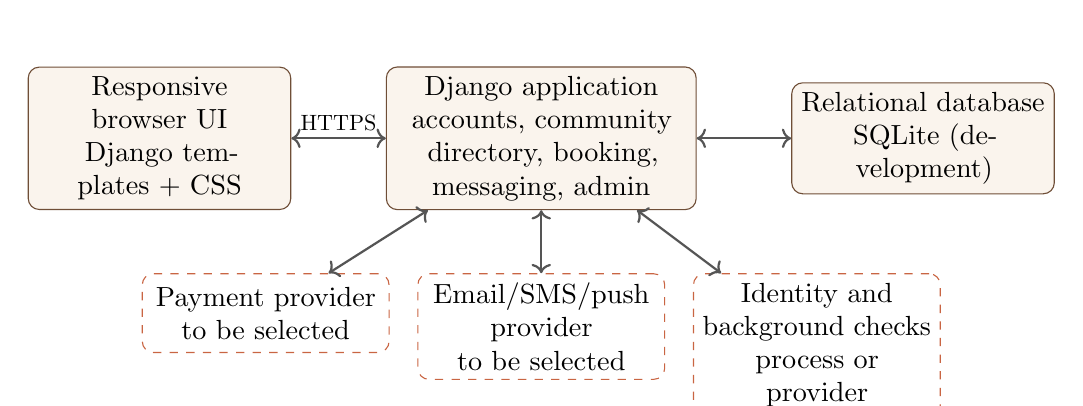
\begin{tikzpicture}[
  node distance=8mm and 12mm,
  box/.style={draw=SabayBrown, rounded corners, align=center, fill=SabayCream, minimum height=10mm, text width=31mm},
  ext/.style={draw=SabayTerracotta, dashed, rounded corners, align=center, minimum height=10mm, text width=29mm},
  arrow/.style={-{Latex[length=2mm]}, thick, draw=SabayGray}
]
  \node[box] (browser) {Responsive browser UI\\Django templates + CSS};
  \node[box, right=of browser, text width=37mm] (app) {Django application\\accounts, community directory, booking, messaging, admin};
  \node[box, right=of app] (db) {Relational database\\SQLite (development)};
  \node[ext, below=of app, xshift=-35mm] (pay) {Payment provider\\to be selected};
  \node[ext, below=of app] (notify) {Email/SMS/push provider\\to be selected};
  \node[ext, below=of app, xshift=35mm] (verify) {Identity and\\background checks\\process or provider};
  \draw[arrow,<->] (browser) -- node[above,scale=.8]{HTTPS} (app);
  \draw[arrow,<->] (app) -- (db);
  \draw[arrow,<->] (app) -- (pay);
  \draw[arrow,<->] (app) -- (notify);
  \draw[arrow,<->] (app) -- (verify);
\end{tikzpicture}
\end{center}

\subsection{Major components}

\begin{tabularx}{\textwidth}{p{0.25\textwidth}X}
\toprule
\textbf{Component} & \textbf{Responsibility} \\
\midrule
Web interface & Responsive views for discovery, profiles, support requests, scheduling, messages, payments, notifications, and administrative work. The current repository supplies only the shared template and placeholder home page. \\
Identity and access & Registration, authentication, role-aware authorization, session security, password policy, and optional or required MFA. Django authentication provides a base but the user experience and policies remain to be built. \\
Community resource directory & Caregiver profiles, service categories, requests for support, search/filtering, matching, reviews, and verification status. \\
Booking & Availability, booking requests, status transitions, cancellations, and one-time or recurring schedules. \\
Messaging and notifications & Booking-scoped conversations and timely new-activity alerts without exposing sensitive content unnecessarily. \\
Payments & Provider-hosted or tokenized checkout, payment state, receipts, refunds, and caregiver payout coordination; sensitive card data should not be stored by Sabay. \\
Administration and trust & Manual caregiver review, evidence handling, moderation, account controls, and operational audit records. \\
Persistence & Relational storage for users and community-platform data. SQLite is configured for development; a production database has not been selected in the supplied artifacts. \\
\bottomrule
\end{tabularx}

\section{How: Development Process}

\subsection{Workflow and tools}

The repository indicates an iterative, issue-driven GitHub workflow using issues and milestones. Pull requests run continuous integration checks for Ruff linting and Django validation, migration drift, and tests. Dependabot proposes dependency updates. A repository Git hook can format Python files with Ruff. Local development uses Python, a virtual environment, Pipenv, Django, SQLite, HTML templates, and Simple.css.

The recommended working loop is: refine a sponsor-validated user story; define acceptance criteria; create and estimate issues; implement in a short-lived branch; add tests; obtain peer review; merge only after CI succeeds; demonstrate the completed slice; and update the backlog and this document. The team should review scope, risk, and progress with the sponsor on a regular cadence.

\subsection{Quality strategy}

Current tests cover routing, successful rendering, template inheritance, and static CSS discovery. As domain features are introduced, the test suite should add model constraints, permission boundaries, form validation, booking state transitions, payment webhooks, notification behavior, and end-to-end tests for the critical user journeys. Security and accessibility review should be included before sponsor delivery.

\subsection{Licensing and intellectual property}

The repository is licensed under the MIT License, matching the sponsor's request. Contributors should only add code, fonts, images, icons, and dependencies whose licenses allow the intended distribution. Mockup testimonials, caregiver identities, claims, certification badges, and prices should be treated as placeholders unless the sponsor confirms they are authorized and accurate. Third-party service terms, privacy obligations, and branding rules must be reviewed before production use.

\subsection{Risks and mitigations}

\begin{longtable}{p{0.24\textwidth}p{0.34\textwidth}p{0.34\textwidth}}
\toprule
\textbf{Risk} & \textbf{Impact} & \textbf{Mitigation} \\
\midrule
Account compromise and weak or reused passwords & Exposure of personal information and fraudulent activity & Use Django's password validators, secure session settings, rate limiting, MFA for sensitive roles, reset/recovery controls, and alerts for suspicious activity. \\
\addlinespace
Authorization defects & One user sees another user's care, booking, or message data & Deny by default; centralize object-level authorization; add negative permission tests for every role and resource. \\
\addlinespace
Sensitive personal data & Privacy, safety, legal, and reputational harm & Minimize collected data, define retention and deletion, encrypt transport and managed storage, restrict staff access, avoid sensitive content in logs/notifications, and complete a privacy/legal review. \\
\addlinespace
Caregiver misrepresentation or unsafe conduct & Physical harm and loss of trust & Define what ``verified'' means, review evidence consistently, show verification limits clearly, support reporting and suspension, and obtain sponsor/legal guidance on checks and insurance. \\
\addlinespace
Payment failure or fraud & Lost funds, disputes, or double charges & Use a reputable processor; do not store card data; verify signed webhooks; make operations idempotent; document cancellations, refunds, payouts, and dispute handling. \\
\addlinespace
Scope exceeds capstone capacity & Core workflows remain incomplete & Validate a thin end-to-end MVP first; rank stories with the sponsor; move native apps and unconfirmed mockup features to the backlog. \\
\addlinespace
Accessibility or usability barriers & Intended users cannot complete core tasks & Test with older and low-technical-confidence users; use WCAG-informed acceptance criteria, readable content, large controls, keyboard support, and clear recovery paths. \\
\addlinespace
DDoS, brute force, and server compromise & Outage or unauthorized access & Use managed hosting/CDN protections where appropriate, application rate limiting, least privilege, patching, hardened SSH or no public SSH, monitoring, backups, and incident procedures. Fail2ban and SSH hardening apply only if the team operates a host directly. \\
\addlinespace
Third-party service delay & Blocks verification, payment, or notifications & Select providers early, isolate integrations behind service interfaces, use sandbox environments, and provide clearly labeled demo substitutes when appropriate. \\
\bottomrule
\end{longtable}

\section{Future Work and Backlog}

\subsection{Likely post-MVP features}

Effort ranges below are rough engineering estimates for a small team after requirements and architecture are stable; they exclude procurement, legal review, and app-store review.

\begin{tabularx}{\textwidth}{X p{0.18\textwidth} X}
\toprule
\textbf{Feature} & \textbf{Rough effort} & \textbf{Notes} \\
\midrule
Check-ins and family updates & 2--4 team-weeks & Define audiences, consent, content, and notification rules. \\
Reminders and task lists & 2--4 team-weeks & Include recurring tasks, acknowledgement, and missed-task behavior. \\
Visit tracking & 3--6 team-weeks & Requires privacy-conscious check-in/out semantics; avoid unnecessary location collection. \\
Emergency-contact workflow & 3--6+ team-weeks & High-risk feature requiring careful language, reliability goals, escalation policy, and legal review; not a substitute for emergency services. \\
Native Android and iOS apps & 8--16+ team-weeks & Depends on API readiness, platform choice, notifications, accessibility, testing, and store delivery. \\
Video interviews & 2--5 team-weeks & Prefer a managed provider; assess privacy, moderation, accessibility, and cost. \\
Optional memberships or subscriptions & 3--6 team-weeks & Consider only if they support sustainability without creating inappropriate barriers to essential community access; confirm entitlements, assistance options, trial/cancellation rules, and prices first. \\
Advanced matching and recommendations & 4--8+ team-weeks & Requires sufficient data, explainable ranking criteria, and bias review. \\
\bottomrule
\end{tabularx}

\subsection{Technical, safety, and legal decisions}

\begin{itemize}
  \item Select hosting, production database/storage, notifications, payments, verification/background checks, monitoring, backups, secrets management, and deployment automation.
  \item Determine authentication and MFA policy, session duration, authorization matrix, audit needs, retention/deletion policy, breach/incident response, and account recovery/support procedure.
  \item Obtain appropriate legal and privacy review for platform liability, caregiver classification, background-check claims, consumer payments, accessibility, minors or vulnerable adults, emergency language, insurance, terms of service, and privacy notice.
  \item Set measurable availability, performance, accessibility, security, browser/device support, and backup/recovery acceptance criteria.
\end{itemize}

\appendix
\section{Glossary of Terms}

\begin{description}[style=nextline]
  \item[Accessibility] Designing and testing the service so people with disabilities can perceive, understand, navigate, and operate it.
  \item[Aging in place] Remaining in one's home and community while receiving the support needed to do so safely.
  \item[Care seeker] A person seeking non-medical support for themself or another person.
  \item[Caregiver/helper] A provider offering the services available through Sabay. The final document should use the sponsor-approved term consistently.
  \item[CI (continuous integration)] Automated checks run when proposed code changes are submitted or updated.
  \item[DDoS] Distributed denial-of-service attack: traffic intended to exhaust a service and make it unavailable.
  \item[Django] The Python web framework used by the current Sabay repository.
  \item[MFA] Multi-factor authentication: account access requiring more than one type of proof.
  \item[MIT License] A permissive open-source software license used by the Sabay repository.
  \item[MVP (minimum viable product)] The smallest sponsor-approved product that delivers the essential end-to-end value and can be evaluated with users.
  \item[Non-medical support] Assistance with daily activities that does not constitute diagnosis, treatment, or another regulated clinical service; the sponsor must define Sabay's precise boundary.
  \item[Responsive website] A web interface that adapts to phone, tablet, and desktop screen sizes.
  \item[Verification] An administrative or third-party review resulting in a clearly defined status; it must not imply guarantees beyond the checks actually performed.
  \item[WCAG] Web Content Accessibility Guidelines, commonly used criteria for accessible web content.
\end{description}

\section{Additional Candidate User Stories}

These stories are candidates for backlog refinement rather than confirmed MVP commitments.

\begin{enumerate}
  \item \textbf{Receive activity notifications.} As a user, I can receive a timely alert for relevant message or booking activity so that I do not miss a change.
  \item \textbf{Manage availability.} As a caregiver, I can mark when I am available so that I receive compatible requests.
  \item \textbf{Manage a booking.} As a care seeker or caregiver, I can accept, decline, reschedule, or cancel a booking under clear rules.
  \item \textbf{Review service.} As a participant in a completed booking, I can leave an appropriate review so that future users have useful trust information.
  \item \textbf{Share family updates.} As an authorized family coordinator, I can receive consented updates so that I can remain informed without taking over daily coordination.
  \item \textbf{Report a concern.} As a user, I can report unsafe or inappropriate activity so that Sabay staff can respond.
  \item \textbf{Moderate an account.} As an administrator, I can restrict or restore an account with a recorded reason so that the community platform can be operated safely.
  \item \textbf{Track a visit.} As an authorized participant, I can see when an agreed visit begins and ends so that the service record is clear.
  \item \textbf{Manage tasks.} As a care seeker or family coordinator, I can define recurring household tasks and see their status.
  \item \textbf{Request data deletion.} As a user, I can request account and eligible personal-data deletion so that I can exercise privacy choices.
\end{enumerate}

\section{Source Materials Reviewed}

\begin{itemize}
  \item \emph{PSU CS Capstone: Guidelines for Project Document} --- required project-document structure and maintenance expectations.
  \item \emph{User Stories} --- user and user-story conventions.
  \item \emph{Project Proposal: Sabay} --- sponsor motivation, requested MVP capabilities, licensing, accessibility, and future direction.
  \item \emph{Sabay Mid-project Meeting} --- authors, cycle, MVP summary, technology choice, process, and initial risk list.
  \item \emph{Sabay design mockups} --- proposed visual language, services, discovery flow, plans, reviews, and trust indicators.
  \item Sabay repository source and history as inspected on August 20, 2026.
\end{itemize}

\end{document}
